\documentclass[10pt]{article}
\label{articlepackage}


\usepackage{soul}
%\usepackage{hyperref}
\usepackage{multicol}

\usepackage{setspace}
%\doublespacing

\usepackage[T1]{fontenc}
\usepackage{ifthen}


\usepackage{bm}
\usepackage{bibentry}
\usepackage{subcaption}

\usepackage{amsmath}
\numberwithin{equation}{section}
\numberwithin{figure}{section}
\numberwithin{table}{section}
\numberwithin{footnote}{section}
\usepackage{mathtools}
\usepackage[inline]{enumitem}
\usepackage{booktabs}
%\usepackage[usenames,dvipsnames,pdftex]{xcolor}
\usepackage{tikz}
\usetikzlibrary{backgrounds,shapes,arrows,positioning,calc,snakes,fit}
\usepgflibrary{decorations.markings}



% \setcounter{section}{-1}

\usepackage{graphicx} % standard package
\usepackage{amsmath} % standard package
\DeclareMathOperator{\sech}{sech}
\newcommand*\diff{\mathop{}\!\mathrm{d}}
\newcommand{\txtd}{\textrm{d}}
\usepackage{amssymb} % useful for double backed letter functions
%%%%%%%%%%%%%%%%%%%%%%%%%%%%%%%%%%%%
\usepackage{amsthm} % used to define theorem objects with command \begin{theorem} etc.
\newtheorem{theorem}{Theorem}[section]
\newtheorem{example}{Example}[subsection]
\newtheorem*{definition}{Definition}
%%%%%%%%%%%%%%%%%%%%%%%%%%%%%%%%%%%%
\newcommand{\eprint}[1]{\href{http://arxiv.org/abs/#1}{#1}}
\usepackage[sort&compress]{natbib}
\bibliographystyle{apsrev} % bibliography package and style
\renewcommand{\bibfont}{\small}
\renewcommand{\citenumfont}[1]{\textbf{#1}}
\renewcommand{\bibnumfmt}[1]{[\color{darkblue}\textbf{#1}\color{black}]}
%%%%%%%%%%%%%%%%%%%%%%%%%%%%%%%%%%%%
\usepackage{listings} % code listing and options
\usepackage{color}
%New colors defined below
\definecolor{codegreen}{rgb}{0,0.6,0}
\definecolor{codegray}{rgb}{0.5,0.5,0.5}
\definecolor{codepurple}{rgb}{0.58,0,0.82}
\definecolor{backcolour}{rgb}{0.95,0.95,0.92}
%Code listing style named "mystyle"
\lstdefinestyle{mystyle}{
  backgroundcolor=\color{backcolour},   commentstyle=\color{codegreen},
  keywordstyle=\color{magenta},
  numberstyle=\tiny\color{codegray},
  stringstyle=\color{codepurple},
  basicstyle=\footnotesize,
  breakatwhitespace=false,
  breaklines=true,
  captionpos=b,
  keepspaces=false,
  numbers=right,
  numbersep=4pt,
  showspaces=false,
  showstringspaces=false,
  showtabs=false,
  tabsize=2
}
\lstset{style=mystyle}

\usepackage[flushmargin, hang]{footmisc}
  \addtolength{\footnotesep}{1mm}
  \setlength{\footnotemargin}{1em}
  \renewcommand{\thefootnote}{\textbf{\arabic{footnote}}}
  \renewcommand\footnoterule{{\hrule height 0.2pt}}

\captionsetup[figure]{labelsep=quad, labelfont=bf, textfont=it, width=0.8\linewidth}


\usepackage{sectsty}
\sectionfont{\color{darkblue}\centering \large \textsc}
\subsectionfont{\color{darkblue}\centering \normalsize \textit}
\subsubsectionfont{\color{darkblue}\centering \small \textit}
\renewcommand\thesection{\arabic{section}}
\renewcommand\thesubsection{\arabic{section}.\arabic{subsection}}
\renewcommand\thefigure{\arabic{section}.\arabic{figure}}
\renewcommand\theequation{{\color{SAEblue}\arabic{section}.\arabic{equation}}}
\usepackage{color}
\definecolor{SAEblue}{rgb}{0, .62, .91}
\definecolor{linkgreen}{RGB}{11, 102, 35}
\definecolor{darkblue}{rgb}{.11, .102, .35}

\usepackage[colorlinks]{hyperref}
\hypersetup{colorlinks=true, urlcolor=linkgreen, citecolor=linkgreen, runcolor=black, menucolor=black, filecolor=black, anchorcolor=black, linkcolor=black}
\theoremstyle{definition}


\theoremstyle{definition}

\renewcommand\vec{\mathbf}
\newcommand{\normord}[1]{\raisebox{0.5pt}{:}\,#1\,\raisebox{0.5pt}{:}}
\newcommand{\dagg}{^{\dagger}}
\newcommand{\pr}{^{\prime}}
\newcommand{\nhat}{\hat{\bm{n}}}
\newcommand{\hamilt}{\mathcal{H}}
\newcommand{\mA}{\mathcal{A}}
\newcommand{\mW}{\mathcal{W}}
\newcommand{\mN}{\mathcal{N}}
\newcommand{\mD}{\mathcal{D}}
\newcommand{\mS}{\mathcal{S}}
\newcommand{\mL}{\mathcal{L}}
\newcommand{\mC}{\mathcal{C}}
\newcommand{\mO}{\mathcal{O}}
\newcommand{\mM}{\mathcal{M}}
\newcommand{\mT}{\mathcal{T}}
\newcommand{\mZ}{\mathcal{Z}}
\newcommand{\mR}{\mathcal{R}}
\newcommand{\II}{\mathbb{I}}
\newcommand{\RR}{\mathbb{R}}
\newcommand{\ZZ}{\mathbb{Z}}
\newcommand{\CC}{\mathbb{C}}
\newcommand{\FF}{\mathbb{F}}
\newcommand{\lie}[1]{\mathcal{L}\left(#1\right)}
\newcommand{\set}[1]{\left\{#1\right\}}
\newcommand{\SO}[1]{\textrm{SO}\left(#1\right)}
\newcommand{\SU}[1]{\textrm{SU}\left(#1\right)}
\newcommand{\Orth}[1]{\textrm{O}\left(#1\right)}
\newcommand{\Uni}[1]{\textrm{U}\left(#1\right)}
\newcommand{\paraskip}{\vspace{10pt}}
\newcommand{\del}{\partial}
\newcommand{\TeG}{\mathcal{T}_e(\mathscr{G})}
\newcommand{\TpM}{\mathcal{T}_p(\mathcal{M})}
\newcommand{\TpMs}{\mathcal{T}^{\star}_p(\mathcal{M})}
\newcommand{\etamn}[1]{\eta#1{\mu \nu}}
\newcommand{\upd}[1]{\text{d}#1 \,}
\newcommand{\ud}{\text{d}}
\newcommand{\group}{\mathscr{G}}
\newcommand{\alge}{\mathfrak{g}}
\newcommand{\twobytwo}[4]{\begin{pmatrix}#1&#2 \\ #3&#4 \end{pmatrix}}
\newcommand{\thrbythr}[3]{\begin{pmatrix}#1 \\ #2 \\ #3\end{pmatrix}}
\newcount\colveccount
\newcommand*\colvec[1]{
        \global\colveccount#1
        \begin{pmatrix}
        \colvecnext
}
\def\colvecnext#1{
        #1
        \global\advance\colveccount-1
        \ifnum\colveccount>0
                \\
                \expandafter\colvecnext
        \else
                \end{pmatrix}
        \fi
}

\newenvironment{Figure}
  {\par\medskip\noindent\minipage{\linewidth}}
  {\endminipage\par\medskip}

\newcommand{\Abs}[1]{\left| #1 \right|}
\newcommand{\tr}{\text{Tr}}

\renewcommand\labelitemi{\raisebox{0.25ex}{\tiny$\bullet$}}
\setenumerate{label=\color{SAEblue}{\textbf{\arabic*}}\color{black})}

\usepackage[labelfont=bf]{caption}
\usepackage[margin=0.8in]{geometry}
\usepackage{fancyhdr}
\pagestyle{fancy}
\lhead{\small\textsc{Three Body Decays}}
\chead{}
\rhead{}
\lfoot{}
\cfoot{\textit{\thepage}}
\rfoot{}

\renewcommand*{\thefootnote}{\fnsymbol{footnote}}
\setcounter{footnote}{1}

\begin{document}
\hrule
\vspace{1pt}
\hrule
\begin{center}
\large\textsc{\color{darkblue}\textbf{The Three Body Decay $\pi_0 \rightarrow \gamma\chi\chi$}}
\vspace{5pt}

\footnotesize\textit{\textbf{J.B.G. Alvey}, Theoretical Particle Physics and Cosmology, King's College London\footnote{\href{mailto:james.alvey@kcl.ac.uk}{james.alvey@kcl.ac.uk}}}
\end{center}
\begin{abstract}
\noindent Set of notes describing the kinematics for the two subsequent on-shell two-body decays $\pi_0 \rightarrow \gamma V$, $V \rightarrow \chi\chi$. The kinematics constrain the masses to lie in the ranges $2 m_\chi < m_V < m_\pi$.
\end{abstract}
\hrule
\tableofcontents
\vspace{5pt}
\hrule
\vspace{1pt}
\hrule
\vspace{10pt}
\renewcommand{\thefootnote}{\tiny\textbf{\arabic{section}.\arabic{footnote}}}
%\begin{multicols*}{2}
\section{The First Decay}
The first decay in the process involves $\pi_0 \rightarrow \gamma V$ where $V$ is some dark vector mediator that kinetically mixes with the standard model photon. In the situation of interest, we have a distribution of pion energies which we wish to translate into a distribution of dark matter energies. Let $p_\mu^\pi$ be the 4-momentum of the pion in the lab frame. We choose our co-ordinate frame such that the pion is propagating along the $z$-axis. In the lab frame, this 4-momenta is given by;
\begin{equation}
  p^\pi_\mu = (E_\pi, 0, 0, \sqrt{E_\pi^2 - m_\pi^2})
\end{equation}
whilst in the rest frame of the pion we have,
\begin{equation}
  p^{\pi, c}_\mu = (m_\pi, \mathbf{0})
\end{equation}
In the rest frame, we can consider the decay as shown in Figure \ref{fig:decay}. The angles $\theta$ and $\phi$ parametrise the decay and should be sampled from suitable distributions. In the implementation of what follows, we take $\phi \in U[0, 2\pi]$ and $\cos\theta \in U[-1, 1]$. Note that this of course does not mean the angles are uniformly distributed in the lab frame since they are boosted in the direction of the pion.
\begin{center}
\begin{figure}
  \centering
  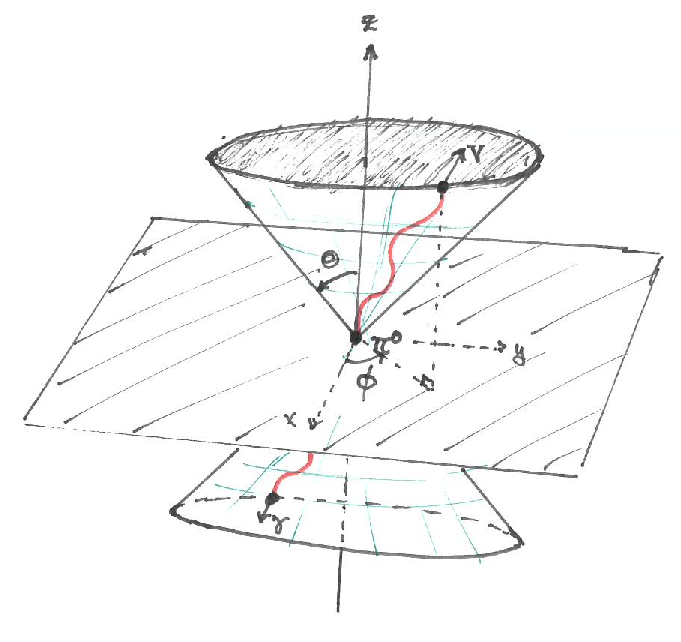
\includegraphics[width=0.5\linewidth]{diag}
  \caption{We parametrise the decay of the $\pi_0$ using two angles, $\theta$ and $\phi$ which ar distributed accordingly.}
  \label{fig:decay}
\end{figure}
\end{center}
\subsection{Energy and Momentum Conservation}
\noindent Conserving energy and momentum in this frame;
\begin{align}
  \sqrt{\Abs{\mathbf{p}_V^c}^2 + m_V^2} + \Abs{\mathbf{p}_\gamma^c} &= m_\pi \\
  \mathbf{p}_V^c &= -\mathbf{p}_\gamma^c
\end{align}
Here the superscript indicates that the quantities are measured in the rest frame of the pion. Substituting the second relation into the first,
\begin{equation}
  \sqrt{\Abs{\mathbf{p}_V^c}^2 + m_V^2} + \Abs{\mathbf{p}_V^c} = m_\pi
\end{equation}
Solving this for $\Abs{\mathbf{p}_V^c}$, we find,
\begin{equation}
  \label{eq:pv}
  \Abs{\mathbf{p}_V^c} := p_V = \frac{m_\pi^2 - m_V^2}{2m_\pi}
\end{equation}
\subsection{Going Back to the Lab Frame}
We now have the 4-momentum for the massive mediator in the pion rest frame via the parametrisation,
\begin{equation}
  p^{V,c}_\mu = (\sqrt{p_V^2 + m_V^2}, p_V\sin\theta\cos\phi, p_V\sin\theta\sin\phi, p_V\cos\theta)
\end{equation}
We can then boost to the lab frame by making a Lorentz transformation with respect to the pion 3-momentum. This leads to a Lorentz transformation of the form,
\begin{equation}
  \Lambda_1 = \begin{pmatrix} \gamma_1 & 0 & 0 & \gamma_1\beta_1 \\ 0 & 1 & 0 & 0 \\ 0 & 0 & 1 & 0 \\ \gamma_1\beta_1 & 0 & 0 & \gamma_1 \end{pmatrix}
\end{equation}
where the $\gamma$ and $\beta$ factors are given as;
\begin{equation}
  \label{eq:gammabeta}
  \gamma_1 = \frac{E_\pi}{m_\pi}, \, \beta_1 = \left(1 - \frac{1}{\gamma^2}\right)^{\frac{1}{2}}
\end{equation}
The 4-momentum of the mediator is then given via $p_\mu^V := (E^V, \mathbf{p}^V) = (\Lambda_1 p^{V, c})_\mu$;
\begin{align}
  E^V &= \gamma_1\sqrt{p_V^2 + m_V^2} + \gamma_1\beta_1p_V\cos\theta \\
  p^V_x &= p_V \sin\theta\cos\phi \label{eq:pvx} \\
  p^V_y &= p_V \sin\theta\sin\phi \\
  p^V_z &= \gamma_1\beta_1\sqrt{p_V^2 + m_V^2} + \gamma_1 p_V \cos\theta \label{eq:pvz}
\end{align}
where $p_V$, $\gamma_1$ and $\beta_1$ are as defined in \eqref{eq:pv} and \eqref{eq:gammabeta}.
\section{The Second Decay}
We need to repeat the process above but for the decay $V \rightarrow \chi\chi$. There will be two differences. Firstly, both the products of the decay have the same mass. Secondly, the mediator $V$ no longer has a $3$-momentum along the $z$ axis so the form of the Lorentz boost will change. We construct an identical diagram to Figure \ref{fig:decay} except we relabel the angles to be $\theta^V$ and $\phi^V$. We let the $4$-momentum of the dark matter particles in the rest frame of $V$ be;
\begin{equation}
  p^{1,c}_\mu = (E_{1}^c, \mathbf{p}^c_{1}), \, p^{2,c}_\mu = (E_{1}^c, -\mathbf{p}^c_{1})
\end{equation}
Now conservation of energy in the rest frame of $V$ gives;
\begin{align}
  \label{eq:pchi}
  2\sqrt{\Abs{p_{1}^c}^2 + m_\chi^2} = m_V \Rightarrow \Abs{\mathbf{p}_{1}^c} := p_\chi = \sqrt{\frac{1}{4}m_V^2 - m_\chi^2}
\end{align}
With the parameterisation given, the 4-momentum of the dark matter particles in the rest frame of $V$ is now given by;
\begin{equation}
  E_{1}^c = \sqrt{p_\chi^2 + m_\chi^2}, \mathbf{p}^c_1 = (p_\chi\sin\theta^V\cos\phi^V, \ldots)
\end{equation}
\subsection{Boosting to the Lab Frame}
The final step is to boost back to the lab frame using a suitable Lorentz transformation. This is determined by the $3$-momentum of the mediator. The Lorentz matrix then takes the form;
\begin{equation}
  \Lambda_2 = \begin{pmatrix} \gamma_2 & \gamma_2\beta_2 \frac{p^V_x}{q_V} & \gamma_2\beta_2 \frac{p^V_y}{q_V} & \gamma_2\beta_2 \frac{p^V_z}{q_V} \\ \gamma_2\beta_2 \frac{p^V_x}{q_V} & 1 + (\gamma_2 - 1)\frac{(p^V_x)^2}{q_V^2} & (\gamma_2 - 1)\frac{p^V_x p^V_y}{q_V^2} & (\gamma_2 - 1)\frac{p^V_x p^V_z}{q_V^2} \\ \gamma_2\beta_2 \frac{p^V_y}{q_V} & (\gamma_2 - 1)\frac{p^V_y p^V_x}{q_V^2} & 1 + (\gamma_2 - 1)\frac{(p^V_y)^2}{q_V^2} & (\gamma_2 - 1)\frac{p^V_y p^V_z}{q_V^2} \\ \gamma_2\beta_2 \frac{p^V_z}{q_V} & (\gamma_2 - 1)\frac{p^V_z p^V_x}{q_V^2} & (\gamma_2 - 1)\frac{p^V_z p^V_y}{q_V^2} & 1 + (\gamma_2 - 1)\frac{(p^V_x)^2}{q_V^2} \end{pmatrix}
\end{equation}
where we have,
\begin{equation}
  \label{eq:g2b2}
  \gamma_2 = \frac{E^V}{m_V}, \, \beta_2 = \left(1 - \frac{1}{\gamma_2^2}\right)^{\frac{1}{2}}, \, q_V = \sqrt{(p_x^V)^2 + (p_y^V)^2 + (p_z^V)^2}
\end{equation}
The energies and 3-momenta of the dark matter particles, in the lab frame of the original $\pi_0$ are then obtained via;
\begin{equation}
p_\mu(\chi_1) = (\Lambda_2 p^{1, c})_\mu, \, p_\mu(\chi_2) = (\Lambda_2 p^{2, c})_\mu
\end{equation}
The resulting energies, $E_\chi^{1, 2}$ can be obtained from the zeroth components, as well as the kinetic energies $T^{1, 2}_\chi = E_\chi^{1, 2} - m_\chi$. Explicitly, we find;
\begin{equation}
  E_{\chi}^{1, 2} = \gamma_2\sqrt{p_\chi^2 + m_\chi^2} \pm \frac{\gamma_2\beta_2p_\chi}{q_V}\left(p^V_x\sin\theta^V \cos\phi^V + p^V_y \sin\theta^V \sin\phi^V + p^V_z\cos\theta^V\right)
\end{equation}
where $p_\chi$ is defined in \eqref{eq:pchi}, $p_V^{x, y, z}$ in \eqref{eq:pvx} - \eqref{eq:pvz}, and $q_V$, $\gamma_2$, $\beta_2$ in \eqref{eq:g2b2}.
%\end{multicols*}
\end{document}
